%% abtex2-modelo-artigo.tex, v-1.9.6 laurocesar
%% Copyright 2012-2016 by abnTeX2 group at http://www.abntex.net.br/ 
%%
%% This work may be distributed and/or modified under the
%% conditions of the LaTeX Project Public License, either version 1.3
%% of this license or (at your option) any later version.
%% The latest version of this license is in
%%   http://www.latex-project.org/lppl.txt
%% and version 1.3 or later is part of all distributions of LaTeX
%% version 2005/12/01 or later.
%%
%% This work has the LPPL maintenance status `maintained'.
%% 
%% The Current Maintainer of this work is the abnTeX2 team, led
%% by Lauro César Araujo. Further information are available on 
%% http://www.abntex.net.br/
%%
%% This work consists of the files abntex2-modelo-artigo.tex and
%% abntex2-modelo-references.bib
%%

% ------------------------------------------------------------------------
% ------------------------------------------------------------------------
% abnTeX2: Modelo de Artigo Acadêmico em conformidade com
% ABNT NBR 6022:2003: Informação e documentação - Artigo em publicação 
% periódica científica impressa - Apresentação
% ------------------------------------------------------------------------
% ------------------------------------------------------------------------

\documentclass[
    % -- opções da classe memoir --
    article,            % indica que é um artigo acadêmico
    11pt,               % tamanho da fonte
    oneside,            % para impressão apenas no recto. Oposto a twoside
    a4paper,            % tamanho do papel. 
    % -- opções da classe abntex2 --
    %chapter=TITLE,     % títulos de capítulos convertidos em letras maiúsculas
    %section=TITLE,     % títulos de seções convertidos em letras maiúsculas
    %subsection=TITLE,  % títulos de subseções convertidos em letras maiúsculas
    %subsubsection=TITLE % títulos de subsubseções convertidos em letras maiúsculas
    % -- opções do pacote babel --
    english,            % idioma adicional para hifenização
    brazil,             % o último idioma é o principal do documento
    sumario=tradicional,
    ]{abntex2}


% ---
% PACOTES
% ---
\usepackage[table,xcdraw]{xcolor}

% ---
% Pacotes fundamentais 
% ---
\usepackage{lmodern}            % Usa a fonte Latin Modern
\usepackage[T1]{fontenc}        % Selecao de codigos de fonte.
\usepackage[utf8]{inputenc}     % Codificacao do documento (conversão automática dos acentos)
\usepackage{indentfirst}        % Indenta o primeiro parágrafo de cada seção.
\usepackage{nomencl}            % Lista de simbolos
\usepackage{color}              % Controle das cores
\usepackage{graphicx}           % Inclusão de gráficos
\usepackage{microtype}          % para melhorias de justificação
% ---
        
% ---
% Pacotes adicionais, usados apenas no âmbito do Modelo Canônico do abnteX2
% ---
\usepackage{lipsum}             % para geração de dummy text
\usepackage{fancyvrb}
\usepackage{todonotes}
\usepackage{float}
\usepackage{listings}
% ---
        
% ---
% Pacotes de citações
% ---
\usepackage[brazilian,hyperpageref]{backref}     % Paginas com as citações na bibl
\usepackage[alf]{abntex2cite}   % Citações padrão ABNT
% ---

% ---
% Configurações do pacote backref
% Usado sem a opção hyperpageref de backref
\renewcommand{\backrefpagesname}{Citado na(s) página(s):~}
% Texto padrão antes do número das páginas
\renewcommand{\backref}{}
% Define os textos da citação
\renewcommand*{\backrefalt}[4]{
    \ifcase #1 %
        Nenhuma citação no texto.%
    \or
        Citado na página #2.%
    \else
        Citado #1 vezes nas páginas #2.%
    \fi}%
% ---

% ---
% Informações de dados para CAPA e FOLHA DE ROSTO
% ---
\titulo{INE5644 - Data Mining\\ 
        Exercício - Árvore de decisão}
\autor{Bruno Marques do Nascimento\thanks{brunomn95@gmail.com \hspace{1mm} - \hspace{1mm} Universidade Federal de Santa Catarina}}
\instituicao{Universidade Federal de Santa Catarina}
\local{Florianópolis - SC, Brasil}
\data{30 de Abril de 2018}
% ---

% ---
% Configurações de aparência do PDF final

% alterando o aspecto da cor azul
\definecolor{blue}{RGB}{41,5,195}

% informações do PDF
\makeatletter
\hypersetup{
        %pagebackref=true,
        pdftitle={\@title}, 
        pdfauthor={\@author},
        pdfsubject={Modelo de artigo científico com abnTeX2},
        pdfcreator={LaTeX with abnTeX2},
        pdfkeywords={abnt}{latex}{abntex}{abntex2}{atigo científico}, 
        colorlinks=true,            % false: boxed links; true: colored links
        linkcolor=blue,             % color of internal links
        citecolor=blue,             % color of links to bibliography
        filecolor=magenta,              % color of file links
        urlcolor=blue,
        bookmarksdepth=4
}
\makeatother
% --- 

% ---
% compila o indice
% ---
\makeindex
% ---

% ---
% Altera as margens padrões
% ---
\setlrmarginsandblock{3cm}{3cm}{*}
\setulmarginsandblock{3cm}{3cm}{*}
\checkandfixthelayout
% ---

% --- 
% Espaçamentos entre linhas e parágrafos 
% --- 

% O tamanho do parágrafo é dado por:
\setlength{\parindent}{1.3cm}

% Controle do espaçamento entre um parágrafo e outro:
\setlength{\parskip}{0.2cm}  % tente também \onelineskip

% Espaçamento simples
\SingleSpacing

% ----
% Início do documento
% ----
\begin{document}

% Seleciona o idioma do documento (conforme pacotes do babel)
%\selectlanguage{english}
\selectlanguage{brazil}

% Retira espaço extra obsoleto entre as frases.
\frenchspacing 

% ----------------------------------------------------------
% ELEMENTOS PRÉ-TEXTUAIS
% ----------------------------------------------------------

%---
%
% Se desejar escrever o artigo em duas colunas, descomente a linha abaixo
% e a linha com o texto ``FIM DE ARTIGO EM DUAS COLUNAS''.
% \twocolumn[           % INICIO DE ARTIGO EM DUAS COLUNAS
%
%---
% página de titulo

\maketitle


% ----------------------------------------------------------
% ELEMENTOS TEXTUAIS
% ----------------------------------------------------------
\textual

% ----------------------------------------------------------
% Introdução
% ----------------------------------------------------------
% \section*{Introdução}
% \addcontentsline{toc}{section}{Introdução}

\section*{\textbf{Respostas:}}
\addcontentsline{toc}{section}{Respostas}

% ----------------------------------------------------------
% Questão 2
% ----------------------------------------------------------
\setcounter{section}{2}
\section*{\textbf{Exercício 2:}}
\addcontentsline{toc}{section}{Exercício 2}

\subsection{\textbf{ID3:}}
\begin{itemize}
  \item Dados:
  \begin{Verbatim}[frame=single, fontsize=\tiny]
  @RELATION cogumelos.venenosos

  @ATTRIBUTE Cor      {Púrpura,Vermelha,Azul}
  @ATTRIBUTE Altura   {Alta,Baixa}
  @ATTRIBUTE Faixas   {Sim,Não}
  @ATTRIBUTE Textura  {Áspera,Suave,Intermediária}
  @ATTRIBUTE Venenoso {Sim,Não}

  @DATA
  Púrpura,   Alta,   Sim,  Áspera,         Sim
  Púrpura,   Alta,   Sim,  Suave,          Sim
  Vermelha,  Baixa,  Sim,  Intermediária,  Não
  Azul,      Baixa,  Não,  Suave,          Não
  Azul,      Baixa,  Sim,  Intermediária,  Sim
  Vermelha,  Alta,   Não,  Intermediária,  Não
  Azul,      Alta,   Sim,  Suave,          Sim
  Azul,      Baixa,  Sim,  Suave,          Sim
  Azul,      Alta,   Não,  Intermediária,  Não
  Azul,      Baixa,  Sim,  Áspera,         Sim
  Vermelha,  Baixa,  Não,  Suave,          Não
  Púrpura,   Baixa,  Não,  Intermediária,  Sim
  Vermelha,  Alta,   Sim,  Intermediária,  Não
  Púrpura,   Alta,   Sim,  Intermediária,  Sim
  Púrpura,   Alta,   Não,  Áspera,         Não
  Púrpura,   Alta,   Não,  Suave,          Não
  \end{Verbatim}
\newpage
  \item Resultado:
  \begin{Verbatim}[frame=single, fontsize=\tiny]
  === Run information ===

  Scheme:       weka.classifiers.trees.Id3 
  Relation:     cogumelos.venenosos
  Instances:    16
  Attributes:   5
                Cor
                Altura
                Faixas
                Textura
                Venenoso
  Test mode:    10-fold cross-validation

  === Classifier model (full training set) ===

  Id3

  Cor = Purpura
  |  Faixas = Sim: Sim
  |  Faixas = Nao
  |  |  Altura = Alta: Nao
  |  |  Altura = Baixa: Sim
  Cor = Vermelha: Nao
  Cor = Azul
  |  Faixas = Sim: Sim
  |  Faixas = Nao: Nao

  Time taken to build model: 0 seconds

  === Stratified cross-validation ===
  === Summary ===

  Correctly Classified Instances          13               81.25   %
  Incorrectly Classified Instances         3               18.75   %
  Kappa statistic                          0.625 
  Mean absolute error                      0.1875
  Root mean squared error                  0.433 
  Relative absolute error                 36.9565 %
  Root relative squared error             85.3206 %
  Total Number of Instances               16     

  === Detailed Accuracy By Class ===

                   TP Rate  FP Rate  Precision  Recall   F-Measure  MCC      ROC Area  PRC Area  Class
                   0,625    0,000    1,000      0,625    0,769      0,674    0,813     0,813     Sim
                   1,000    0,375    0,727      1,000    0,842      0,674    0,813     0,727     Nao
  Weighted Avg.    0,813    0,188    0,864      0,813    0,806      0,674    0,813     0,770     

  === Confusion Matrix ===

   a b   <-- classified as
   5 3 | a = Sim
   0 8 | b = Nao
  \end{Verbatim}

  \item Tempo de construção: \textbf{0 segundos.}
  
  \item Características:
  \begin{itemize}
    \item Altura: 3
    \item Nodos por nível:
    \begin{itemize}
      \item Nível 1: \textbf{1 nodo.}
      \item Nível 2: \textbf{3 nodos.}
      \item Nível 3: \textbf{4 nodos.}
      \item Nível 4: \textbf{2 nodos.}
    \end{itemize}
  \end{itemize}
\end{itemize}   

\newpage
\subsection{\textbf{J48 - Unpruned:}}
\begin{itemize}
  \item Dados:
  \begin{Verbatim}[frame=single, fontsize=\tiny]
  @RELATION cogumelos.venenosos

  @ATTRIBUTE Cor      {Púrpura,Vermelha,Azul}
  @ATTRIBUTE Altura   {Alta,Baixa}
  @ATTRIBUTE Faixas   {Sim,Não}
  @ATTRIBUTE Textura  {Áspera,Suave,Intermediária}
  @ATTRIBUTE Venenoso {Sim,Não}

  @DATA
  Púrpura,   Alta,   Sim,  Áspera,         Sim
  Púrpura,   Alta,   Sim,  Suave,          Sim
  Vermelha,  Baixa,  Sim,  Intermediária,  Não
  Azul,      Baixa,  Não,  Suave,          Não
  Azul,      Baixa,  Sim,  Intermediária,  Sim
  Vermelha,  Alta,   Não,  Intermediária,  Não
  Azul,      Alta,   Sim,  Suave,          Sim
  Azul,      Baixa,  Sim,  Suave,          Sim
  Azul,      Alta,   Não,  Intermediária,  Não
  Azul,      Baixa,  Sim,  Áspera,         Sim
  Vermelha,  Baixa,  Não,  Suave,          Não
  Púrpura,   Baixa,  Não,  Intermediária,  Sim
  Vermelha,  Alta,   Sim,  Intermediária,  Não
  Púrpura,   Alta,   Sim,  Intermediária,  Sim
  Púrpura,   Alta,   Não,  Áspera,         Não
  Púrpura,   Alta,   Não,  Suave,          Não
  \end{Verbatim}

  \item Resultado:
  \begin{Verbatim}[frame=single, fontsize=\tiny]
  === Run information ===

  Scheme:       weka.classifiers.trees.J48 -U -M 2
  Relation:     cogumelos.venenosos
  Instances:    16
  Attributes:   5
                Cor
                Altura
                Faixas
                Textura
                Venenoso
  Test mode:    10-fold cross-validation

  === Classifier model (full training set) ===

  J48 unpruned tree
  ------------------

  Faixas = Sim
  |   Cor = Purpura: Sim (3.0)
  |   Cor = Vermelha: Nao (2.0)
  |   Cor = Azul: Sim (4.0)
  Faixas = Nao: Nao (7.0/1.0)

  Number of Leaves  :     4

  Size of the tree :  6


  Time taken to build model: 0 seconds

  === Stratified cross-validation ===
  === Summary ===

  Correctly Classified Instances          15               93.75   %
  Incorrectly Classified Instances         1                6.25   %
  Kappa statistic                          0.875 
  Mean absolute error                      0.1146
  Root mean squared error                  0.2668
  Relative absolute error                 22.5845 %
  Root relative squared error             52.5695 %
  Total Number of Instances               16     

  === Detailed Accuracy By Class ===

                   TP Rate  FP Rate  Precision  Recall   F-Measure  MCC      ROC Area  PRC Area  Class
                   0,875    0,000    1,000      0,875    0,933      0,882    0,898     0,938     Sim
                   1,000    0,125    0,889      1,000    0,941      0,882    0,898     0,837     Nao
  Weighted Avg.    0,938    0,063    0,944      0,938    0,937      0,882    0,898     0,887     

  === Confusion Matrix ===

   a b   <-- classified as
   7 1 | a = Sim
   0 8 | b = Nao
  \end{Verbatim}

  \item Tempo de construção: \textbf{0 segundos.}
  \item Características:
  \begin{itemize}
    \item Altura: 2
    \item Nodos por nível:
    \begin{itemize}
      \item Nível 1: \textbf{1 nodo.}
      \item Nível 2: \textbf{2 nodos.}
      \item Nível 3: \textbf{3 nodos.}
    \end{itemize}
  \end{itemize}
\end{itemize}

\subsection{\textbf{Árvore de decisão:}}
\begin{itemize}
  \item Árvore de decisão ID3:
  \begin{figure}[H]
      \centering
      \label{id3-decision-tree}
      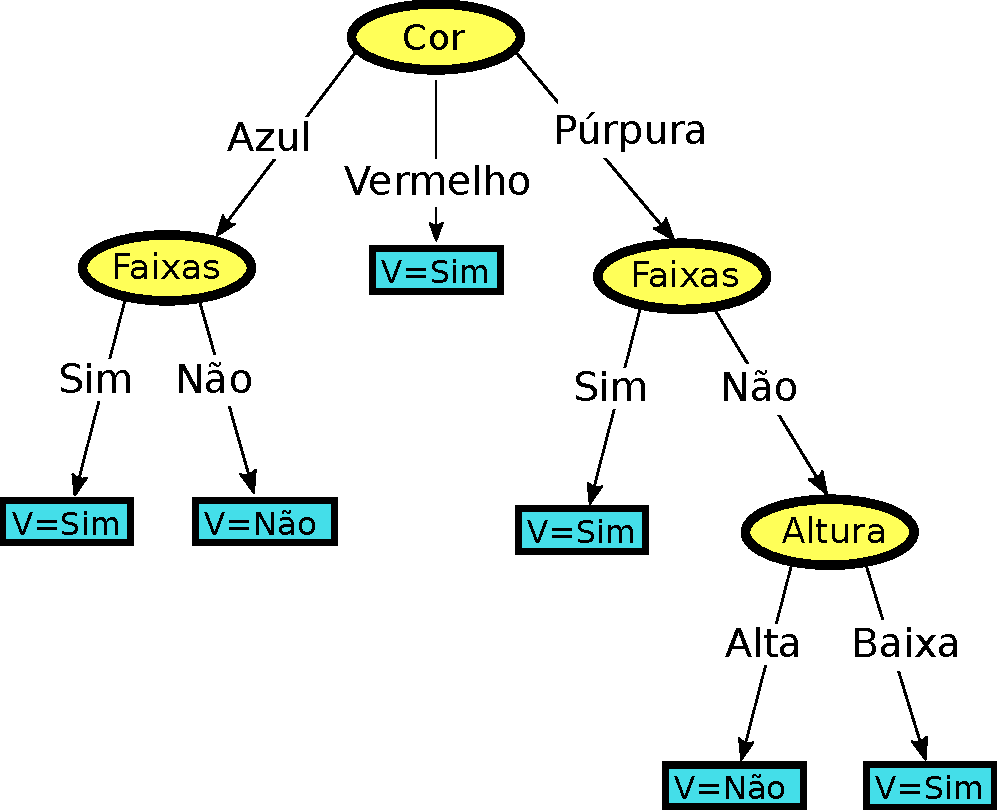
\includegraphics[width=0.5  \textwidth]{imgs/exer2-id3-tree.pdf}
  \end{figure}

  \item Árvore de decisão J48 - Unpruned:
  \begin{figure}[H]
    \centering
    \label{j48-decision-tree}
    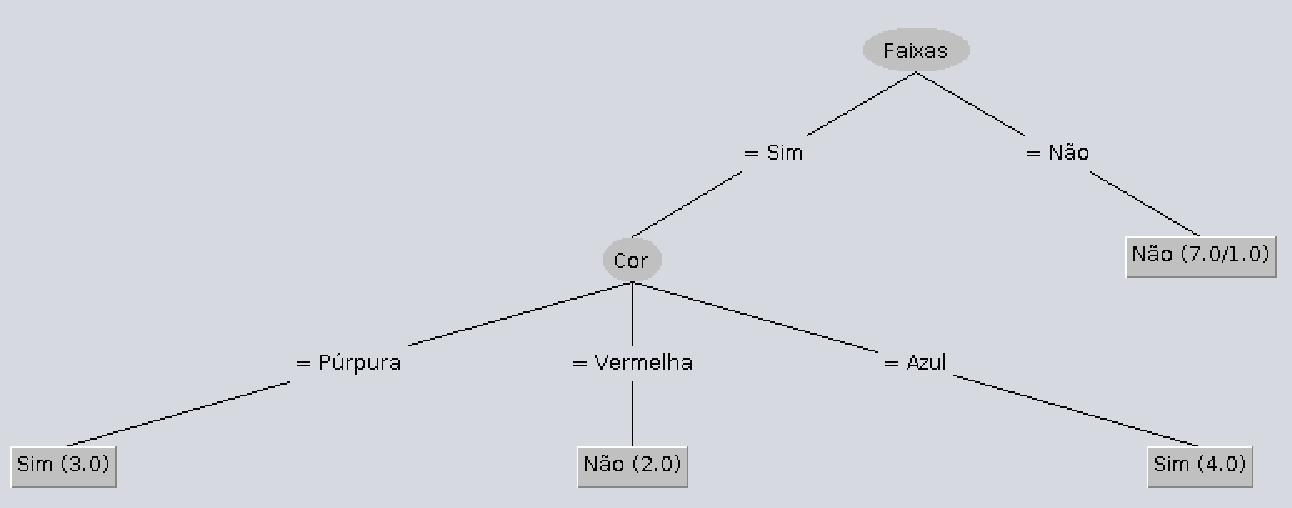
\includegraphics[width=\textwidth]{imgs/exer2-j48-tree.pdf}
  \end{figure}
\end{itemize}

% ----------------------------------------------------------
% Questão 3
% ----------------------------------------------------------
\setcounter{section}{3}
\section*{\textbf{Exercício 3:}}
\addcontentsline{toc}{section}{Exercício 3}

\setcounter{subsection}{0}
\subsection{\textbf{ID3:}}

\begin{itemize}
  \item Dados:
  \begin{Verbatim}[frame=single, fontsize=\tiny]
  @RELATION abordar.motorista

  @ATTRIBUTE UsandoTelefone {Sim,Não}
  @ATTRIBUTE Luzes          {Funcionando, Queimadas}
  @ATTRIBUTE Velocidade     {Lenta,Rápida,Normal}
  @ATTRIBUTE Direcao        {Arriscada,Perigosa,Segura}
  @ATTRIBUTE Abordar        {Sim,Não}

  @DATA
  Sim   Funcionando   Lenta    Arriscada   Não
  Não   Queimadas     Rápida   Perigosa    Sim
  Não   Queimadas     Lenta    Segura      Sim
  Não   Funcionando   Rápida   Arriscada   Não
  Sim   Funcionando   Normal   Perigosa    Não
  Sim   Funcionando   Rápida   Perigosa    Sim
  Não   Queimadas     Lenta    Segura      Sim
  Sim   Queimadas     Rápida   Arriscada   Sim
  Não   Funcionando   Normal   Segura      Não
  Sim   Queimadas     Normal   Arriscada   Sim
  Sim   Queimadas     Lenta    Arriscada   Sim
  Não   Funcionando   Lenta    Segura      Não
  Não   Queimadas     Lenta    Arriscada   Sim
  Sim   Funcionando   Normal   Segura      Não
  Não   Funcionando   Normal   Arriscada   Não
  Não   Funcionando   Lenta    Perigosa    Sim
  Não   Funcionando   Rápida   Segura      Não
  \end{Verbatim}  
  
  \item Resultado:  
  \begin{Verbatim}[frame=single, fontsize=\tiny]
  === Run information ===

  Scheme:       weka.classifiers.trees.Id3 
  Relation:     abordar.motorista
  Instances:    17
  Attributes:   5
                UsandoTelefone
                Luzes
                Velocidade
                Direcao
                Abordar
  Test mode:    10-fold cross-validation

  === Classifier model (full training set) ===

  Id3


  Luzes = Funcionando
  |  Direcao = Arriscada: Não
  |  Direcao = Perigosa
  |  |  Velocidade = Lenta: Sim
  |  |  Velocidade = Rápida: Sim
  |  |  Velocidade = Normal: Não
  |  Direcao = Segura: Não
  Luzes = Queimadas: Sim

  Time taken to build model: 0 seconds

  === Stratified cross-validation ===
  === Summary ===

  Correctly Classified Instances          15               88.2353 %
  Incorrectly Classified Instances         2               11.7647 %
  Kappa statistic                          0.7639
  Mean absolute error                      0.1176
  Root mean squared error                  0.343 
  Relative absolute error                 23.3766 %
  Root relative squared error             68.0355 %
  Total Number of Instances               17     

  === Detailed Accuracy By Class ===

                   TP Rate  FP Rate  Precision  Recall   F-Measure  MCC      ROC Area  PRC Area  Class
                   0,889    0,125    0,889      0,889    0,889      0,764    0,882     0,849     Sim
                   0,875    0,111    0,875      0,875    0,875      0,764    0,882     0,824     Não
  Weighted Avg.    0,882    0,118    0,882      0,882    0,882      0,764    0,882     0,837     

  === Confusion Matrix ===

   a b   <-- classified as
   8 1 | a = Sim
   1 7 | b = Não
  \end{Verbatim}
  \item Tempo de construção: \textbf{0 segundos.}
  \item Características:
  \begin{itemize}
    \item Altura: 3
    \item Nodos por nível:
    \begin{itemize}
      \item Nível 1: \textbf{1 nodo.}
      \item Nível 2: \textbf{2 nodos.}
      \item Nível 3: \textbf{3 nodos.}
      \item Nível 4: \textbf{3 nodos.}
    \end{itemize}
  \end{itemize}
\end{itemize} 


\subsection{\textbf{J48 - Unpruned:}}
\begin{itemize}
  \item Dados:
  \begin{Verbatim}[frame=single, fontsize=\tiny]
  @RELATION abordar.motorista

  @ATTRIBUTE UsandoTelefone {Sim,Não}
  @ATTRIBUTE Luzes          {Funcionando, Queimadas}
  @ATTRIBUTE Velocidade     {Lenta,Rápida,Normal}
  @ATTRIBUTE Direcao        {Arriscada,Perigosa,Segura}
  @ATTRIBUTE Abordar        {Sim,Não}

  @DATA
  Sim   Funcionando   Lenta    Arriscada   Não
  Não   Queimadas     Rápida   Perigosa    Sim
  Não   Queimadas     Lenta    Segura      Sim
  Não   Funcionando   Rápida   Arriscada   Não
  Sim   Funcionando   Normal   Perigosa    Não
  Sim   Funcionando   Rápida   Perigosa    Sim
  Não   Queimadas     Lenta    Segura      Sim
  Sim   Queimadas     Rápida   Arriscada   Sim
  Não   Funcionando   Normal   Segura      Não
  Sim   Queimadas     Normal   Arriscada   Sim
  Sim   Queimadas     Lenta    Arriscada   Sim
  Não   Funcionando   Lenta    Segura      Não
  Não   Queimadas     Lenta    Arriscada   Sim
  Sim   Funcionando   Normal   Segura      Não
  Não   Funcionando   Normal   Arriscada   Não
  Não   Funcionando   Lenta    Perigosa    Sim
  Não   Funcionando   Rápida   Segura      Não
  \end{Verbatim}  
  
  \item Resultado: 
  \begin{Verbatim}[frame=single, fontsize=\tiny]
  === Run information ===

  Scheme:       weka.classifiers.trees.J48 -U -M 2
  Relation:     abordar.motorista
  Instances:    17
  Attributes:   5
                UsandoTelefone
                Luzes
                Velocidade
                Direcao
                Abordar
  Test mode:    10-fold cross-validation

  === Classifier model (full training set) ===

  J48 unpruned tree
  ------------------

  Luzes = Funcionando
  |   Direcao = Arriscada: Não (3.0)
  |   Direcao = Perigosa: Sim (3.0/1.0)
  |   Direcao = Segura: Não (4.0)
  Luzes = Queimadas: Sim (7.0)

  Number of Leaves  :     4

  Size of the tree :  6


  Time taken to build model: 0.01 seconds

  === Stratified cross-validation ===
  === Summary ===

  Correctly Classified Instances          15               88.2353 %
  Incorrectly Classified Instances         2               11.7647 %
  Kappa statistic                          0.7639
  Mean absolute error                      0.1176
  Root mean squared error                  0.3237
  Relative absolute error                 23.3766 %
  Root relative squared error             64.2071 %
  Total Number of Instances               17     

  === Detailed Accuracy By Class ===

                   TP Rate  FP Rate  Precision  Recall   F-Measure  MCC      ROC Area  PRC Area  Class
                   0,889    0,125    0,889      0,889    0,889      0,764    0,924     0,881     Sim
                   0,875    0,111    0,875      0,875    0,875      0,764    0,924     0,918     Não
  Weighted Avg.    0,882    0,118    0,882      0,882    0,882      0,764    0,924     0,899     

  === Confusion Matrix ===

   a b   <-- classified as
   8 1 | a = Sim
   1 7 | b = Não
  \end{Verbatim} 
    
  \item Tempo de construção: \textbf{0.01 segundos.}
  \item Características:
  \begin{itemize}
      \item Altura: 2
      \item Nodos por nível:
          \begin{itemize}
              \item Nível 1: \textbf{1 nodo.}
              \item Nível 2: \textbf{2 nodos.}
              \item Nível 3: \textbf{3 nodos.}
          \end{itemize}
  \end{itemize}
\end{itemize}

\newpage
\subsection{\textbf{Ávore de decisão:}}
\begin{itemize}
  \item Árvore de decisão ID3:
  \begin{figure}[H]
    \centering     
    \label{id3-decision-tree-2}
    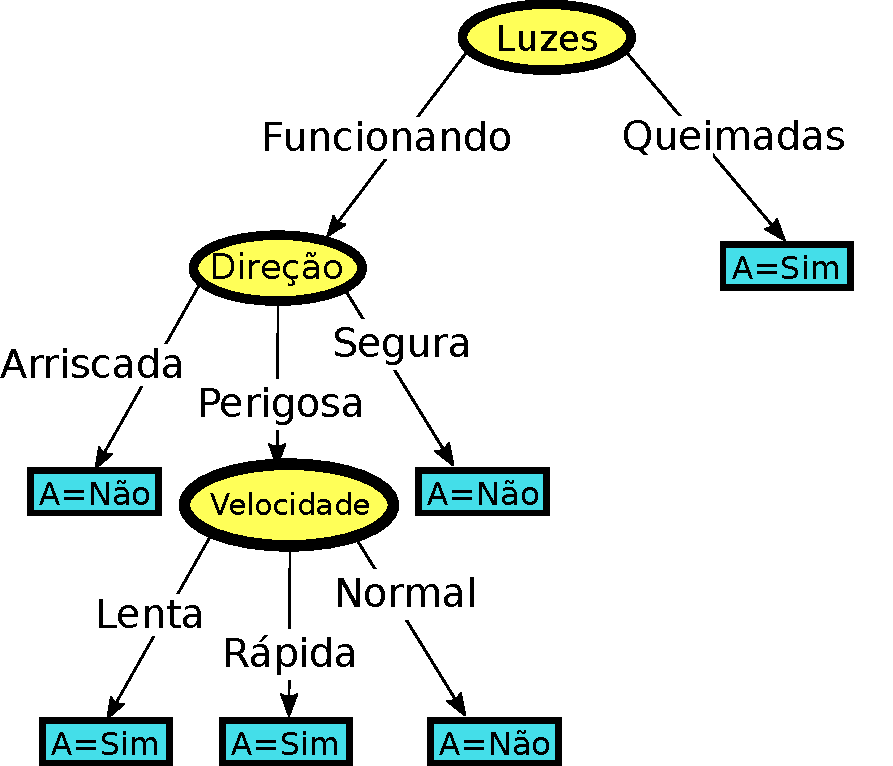
\includegraphics[width=0.5\textwidth]{imgs/exer3-id3-tree.pdf}
  \end{figure}

  \item Árvore de decisão J48 - Unpruned:
  \begin{figure}[H]
    \centering     
    \label{j48-decision-tree-2}
    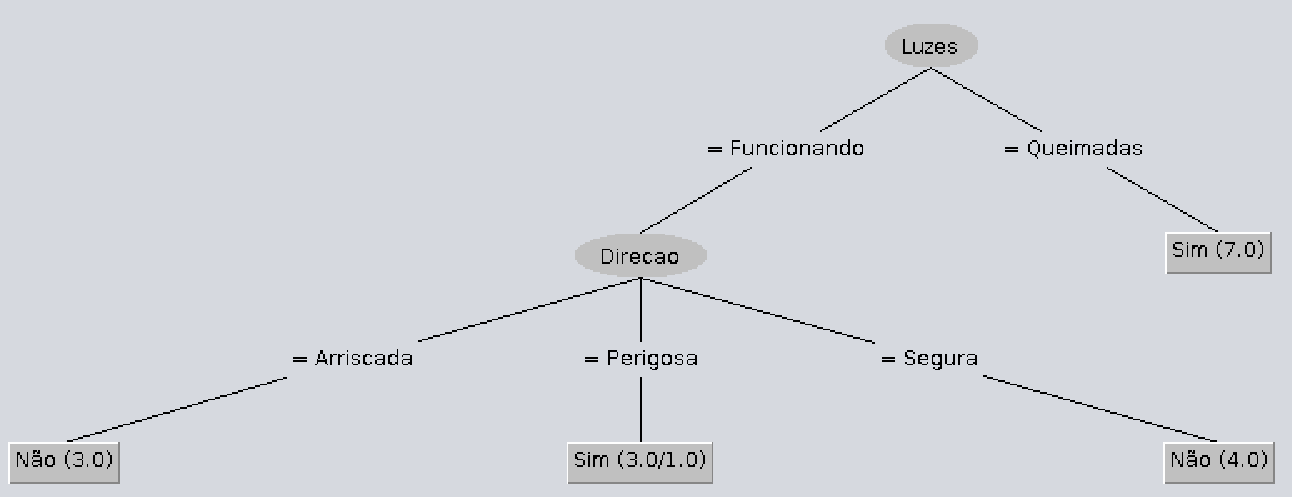
\includegraphics[width=\textwidth]{imgs/exer3-j48-tree.pdf}
  \end{figure}
\end{itemize}  

% ----------------------------------------------------------
% Questão 4
% ----------------------------------------------------------
\newpage
\setcounter{section}{4}
\section*{\textbf{Exercício 4:}}
\addcontentsline{toc}{section}{Exercício 4}

\setcounter{subsection}{0}
\subsection{\textbf{ID3:}}

\subsubsection{\textbf{Exemplo padrão:}}

\begin{itemize}
  \item Dados:
  \begin{Verbatim}[frame=single, fontsize=\tiny]
  @RELATION exemplo.aula

  @ATTRIBUTE montante   {baixo,médio,alto}
  @ATTRIBUTE idade      {jovem,média,sênior}
  @ATTRIBUTE salário    {baixo,alto}
  @ATTRIBUTE conta      {sim,não}
  @ATTRIBUTE empréstimo {sim,não}

  @DATA
  médio   sênior   baixo   sim   não 
  médio   sênior   baixo   não   não 
  baixo   sênior   baixo   sim   sim 
  alto    média    baixo   sim   sim 
  alto    jovem    alto    sim   sim 
  alto    jovem    alto    não   não 
  baixo   jovem    alto    não   sim 
  médio   média    baixo   sim   não 
  médio   jovem    alto    sim   sim 
  alto    média    alto    sim   sim 
  médio   média    alto    não   sim 
  baixo   jovem    baixo   não   sim 
  baixo   sênior   alto    sim   sim 
  alto    média    baixo   não   não 
  \end{Verbatim}
  
  \item Resultado:
  \begin{Verbatim}[frame=single, fontsize=\tiny]
  === Run information ===

  Scheme:       weka.classifiers.trees.Id3 
  Relation:     exemplo.aula
  Instances:    14
  Attributes:   5
                montante
                idade
                salário
                conta
                empréstimo
  Test mode:    10-fold cross-validation

  === Classifier model (full training set) ===

  Id3


  montante = baixo: sim
  montante = médio
  |  salário = baixo: não
  |  salário = alto: sim
  montante = alto
  |  conta = sim: sim
  |  conta = não: não

  Time taken to build model: 0 seconds

  === Stratified cross-validation ===
  === Summary ===

  Correctly Classified Instances          12               85.7143 %
  Incorrectly Classified Instances         2               14.2857 %
  Kappa statistic                          0.6889
  Mean absolute error                      0.1429
  Root mean squared error                  0.378 
  Relative absolute error                 30      %
  Root relative squared error             76.6097 %
  Total Number of Instances               14     

  === Detailed Accuracy By Class ===

                   TP Rate  FP Rate  Precision  Recall   F-Measure  MCC      ROC Area  PRC Area  Class
                   0,889    0,200    0,889      0,889    0,889      0,689    0,844     0,862     sim
                   0,800    0,111    0,800      0,800    0,800      0,689    0,844     0,711     não
  Weighted Avg.    0,857    0,168    0,857      0,857    0,857      0,689    0,844     0,808     

  === Confusion Matrix ===

   a b   <-- classified as
   8 1 | a = sim
   1 4 | b = não
   \end{Verbatim}
\end{itemize}


\subsubsection{\textbf{Exemplo modificado 1:}}

\begin{itemize}
  \item Dados:\\
  Conjunto de dados agrupados/ordenados pelo atributo \texttt{montante}.
  \begin{Verbatim}[frame=single, fontsize=\tiny]
  @RELATION exemplo.aula.modificado1

  @ATTRIBUTE montante   {baixo,médio,alto}
  @ATTRIBUTE idade      {jovem,média,sênior}
  @ATTRIBUTE salário    {baixo,alto}
  @ATTRIBUTE conta      {sim,não}
  @ATTRIBUTE empréstimo {sim,não}

  @DATA
  alto    média    baixo   sim   sim 
  alto    jovem    alto    sim   sim 
  alto    jovem    alto    não   não 
  alto    média    alto    sim   sim 
  alto    média    baixo   não   não 
  médio   sênior   baixo   sim   não 
  médio   sênior   baixo   não   não 
  médio   média    baixo   sim   não 
  médio   jovem    alto    sim   sim 
  médio   média    alto    não   sim 
  baixo   jovem    alto    não   sim 
  baixo   sênior   baixo   sim   sim 
  baixo   jovem    baixo   não   sim 
  baixo   sênior   alto    sim   sim 
  \end{Verbatim}
  
  \item Resultado:
  \begin{Verbatim}[frame=single, fontsize=\tiny]
  === Run information ===

  Scheme:       weka.classifiers.trees.Id3 
  Relation:     exemplo.aula.modificado1
  Instances:    14
  Attributes:   5
                montante
                idade
                salário
                conta
                empréstimo
  Test mode:    10-fold cross-validation

  === Classifier model (full training set) ===

  Id3


  montante = baixo: sim
  montante = médio
  |  salário = baixo: não
  |  salário = alto: sim
  montante = alto
  |  conta = sim: sim
  |  conta = não: não

  Time taken to build model: 0 seconds

  === Stratified cross-validation ===
  === Summary ===

  Correctly Classified Instances          10               71.4286 %
  Incorrectly Classified Instances         4               28.5714 %
  Kappa statistic                          0.3778
  Mean absolute error                      0.2857
  Root mean squared error                  0.5345
  Relative absolute error                 60      %
  Root relative squared error            108.3425 %
  Total Number of Instances               14     

  === Detailed Accuracy By Class ===

                   TP Rate  FP Rate  Precision  Recall   F-Measure  MCC      ROC Area  PRC Area  Class
                   0,778    0,400    0,778      0,778    0,778      0,378    0,689     0,748     sim
                   0,600    0,222    0,600      0,600    0,600      0,378    0,689     0,503     não
  Weighted Avg.    0,714    0,337    0,714      0,714    0,714      0,378    0,689     0,660     

  === Confusion Matrix ===

   a b   <-- classified as
   7 2 | a = sim
   2 3 | b = não
   \end{Verbatim}
\end{itemize}


\subsubsection{\textbf{Exemplo modificado 2:}}

\begin{itemize}
  \item Dados:\\
  Conjunto de dados agrupados/ordenados pelo atributo \texttt{idade}.
  \begin{Verbatim}[frame=single, fontsize=\tiny]
  @RELATION exemplo.aula.modificado2

  @ATTRIBUTE montante   {baixo,médio,alto}
  @ATTRIBUTE idade      {jovem,média,sênior}
  @ATTRIBUTE salário    {baixo,alto}
  @ATTRIBUTE conta      {sim,não}
  @ATTRIBUTE empréstimo {sim,não}

  @DATA
  baixo   jovem    baixo   não   sim 
  alto    jovem    alto    sim   sim 
  alto    jovem    alto    não   não 
  baixo   jovem    alto    não   sim 
  médio   jovem    alto    sim   sim 
  médio   média    baixo   sim   não 
  alto    média    baixo   sim   sim 
  alto    média    alto    sim   sim 
  médio   média    alto    não   sim 
  alto    média    baixo   não   não 
  médio   sênior   baixo   sim   não 
  médio   sênior   baixo   não   não 
  baixo   sênior   baixo   sim   sim 
  baixo   sênior   alto    sim   sim 
  \end{Verbatim}
  
  \item Resultado:
  \begin{Verbatim}[frame=single, fontsize=\tiny]
  === Run information ===

  Scheme:       weka.classifiers.trees.Id3 
  Relation:     exemplo.aula.modificado2
  Instances:    14
  Attributes:   5
                montante
                idade
                salário
                conta
                empréstimo
  Test mode:    10-fold cross-validation

  === Classifier model (full training set) ===

  Id3


  montante = baixo: sim
  montante = médio
  |  salário = baixo: não
  |  salário = alto: sim
  montante = alto
  |  conta = sim: sim
  |  conta = não: não

  Time taken to build model: 0 seconds

  === Stratified cross-validation ===
  === Summary ===

  Correctly Classified Instances          11               78.5714 %
  Incorrectly Classified Instances         1                7.1429 %
  Kappa statistic                          0.8   
  Mean absolute error                      0.0833
  Root mean squared error                  0.2887
  Relative absolute error                 20.5882 %
  Root relative squared error             63.7922 %
  UnClassified Instances                   2               14.2857 %
  Total Number of Instances               14     

  === Detailed Accuracy By Class ===

                   TP Rate  FP Rate  Precision  Recall   F-Measure  MCC      ROC Area  PRC Area  Class
                   1,000    0,250    0,889      1,000    0,941      0,816    0,844     0,862     sim
                   0,750    0,000    1,000      0,750    0,857      0,816    0,800     0,743     não
  Weighted Avg.    0,917    0,167    0,926      0,917    0,913      0,816    0,830     0,822     

  === Confusion Matrix ===

   a b   <-- classified as
   8 0 | a = sim
   1 3 | b = não
  \end{Verbatim}
\end{itemize}

\subsection{\textbf{J48 - Unpruned:}}

\subsubsection{\textbf{Exemplo padrão:}}
\begin{itemize}
  \item Dados:
  \begin{Verbatim}[frame=single, fontsize=\tiny]
  @RELATION exemplo.aula

  @ATTRIBUTE montante   {baixo,médio,alto}
  @ATTRIBUTE idade      {jovem,média,sênior}
  @ATTRIBUTE salário    {baixo,alto}
  @ATTRIBUTE conta      {sim,não}
  @ATTRIBUTE empréstimo {sim,não}

  @DATA
  médio   sênior   baixo   sim   não 
  médio   sênior   baixo   não   não 
  baixo   sênior   baixo   sim   sim 
  alto    média    baixo   sim   sim 
  alto    jovem    alto    sim   sim 
  alto    jovem    alto    não   não 
  baixo   jovem    alto    não   sim 
  médio   média    baixo   sim   não 
  médio   jovem    alto    sim   sim 
  alto    média    alto    sim   sim 
  médio   média    alto    não   sim 
  baixo   jovem    baixo   não   sim 
  baixo   sênior   alto    sim   sim 
  alto    média    baixo   não   não 
  \end{Verbatim}

  \item Resultado:
  \begin{Verbatim}[frame=single, fontsize=\tiny]
  === Run information ===

  Scheme:       weka.classifiers.trees.J48 -U -M 2
  Relation:     exemplo.aula
  Instances:    14
  Attributes:   5
                montante
                idade
                salário
                conta
                empréstimo
  Test mode:    10-fold cross-validation

  === Classifier model (full training set) ===

  J48 unpruned tree
  ------------------

  montante = baixo: sim (4.0)
  montante = médio
  |   salário = baixo: não (3.0)
  |   salário = alto: sim (2.0)
  montante = alto
  |   conta = sim: sim (3.0)
  |   conta = não: não (2.0)

  Number of Leaves  :     5

  Size of the tree :  8


  Time taken to build model: 0 seconds

  === Stratified cross-validation ===
  === Summary ===

  Correctly Classified Instances           8               57.1429 %
  Incorrectly Classified Instances         6               42.8571 %
  Kappa statistic                          0.0667
  Mean absolute error                      0.369 
  Root mean squared error                  0.5713
  Relative absolute error                 77.5    %
  Root relative squared error            115.7978 %
  Total Number of Instances               14     

  === Detailed Accuracy By Class ===

                   TP Rate  FP Rate  Precision  Recall   F-Measure  MCC      ROC Area  PRC Area  Class
                   0,667    0,600    0,667      0,667    0,667      0,067    0,689     0,792     sim
                   0,400    0,333    0,400      0,400    0,400      0,067    0,689     0,486     não
  Weighted Avg.    0,571    0,505    0,571      0,571    0,571      0,067    0,689     0,683     

  === Confusion Matrix ===

   a b   <-- classified as
   6 3 | a = sim
   3 2 | b = não
  \end{Verbatim}
\end{itemize}

\subsubsection{\textbf{Exemplo modificado 1:}}
\begin{itemize}
  \item Dados:\\
  Conjunto de dados agrupados/ordenados pelo atributo \texttt{montante}.
  \begin{Verbatim}[frame=single, fontsize=\tiny]
  @RELATION exemplo.aula.modificado1

  @ATTRIBUTE montante   {baixo,médio,alto}
  @ATTRIBUTE idade      {jovem,média,sênior}
  @ATTRIBUTE salário    {baixo,alto}
  @ATTRIBUTE conta      {sim,não}
  @ATTRIBUTE empréstimo {sim,não}

  @DATA
  alto    média    baixo   sim   sim 
  alto    jovem    alto    sim   sim 
  alto    jovem    alto    não   não 
  alto    média    alto    sim   sim 
  alto    média    baixo   não   não 
  médio   sênior   baixo   sim   não 
  médio   sênior   baixo   não   não 
  médio   média    baixo   sim   não 
  médio   jovem    alto    sim   sim 
  médio   média    alto    não   sim 
  baixo   jovem    alto    não   sim 
  baixo   sênior   baixo   sim   sim 
  baixo   jovem    baixo   não   sim 
  baixo   sênior   alto    sim   sim 
  \end{Verbatim}

  \item Resultado:
  \begin{Verbatim}[frame=single, fontsize=\tiny]
  === Run information ===

  Scheme:       weka.classifiers.trees.J48 -U -M 2
  Relation:     exemplo.aula.modificado1
  Instances:    14
  Attributes:   5
                montante
                idade
                salário
                conta
                empréstimo
  Test mode:    10-fold cross-validation

  === Classifier model (full training set) ===

  J48 unpruned tree
  ------------------

  montante = baixo: sim (4.0)
  montante = médio
  |   salário = baixo: não (3.0)
  |   salário = alto: sim (2.0)
  montante = alto
  |   conta = sim: sim (3.0)
  |   conta = não: não (2.0)

  Number of Leaves  :     5

  Size of the tree :  8


  Time taken to build model: 0 seconds

  === Stratified cross-validation ===
  === Summary ===

  Correctly Classified Instances           8               57.1429 %
  Incorrectly Classified Instances         6               42.8571 %
  Kappa statistic                          0.1429
  Mean absolute error                      0.375 
  Root mean squared error                  0.5586
  Relative absolute error                 78.75   %
  Root relative squared error            113.2173 %
  Total Number of Instances               14     

  === Detailed Accuracy By Class ===

                   TP Rate  FP Rate  Precision  Recall   F-Measure  MCC      ROC Area  PRC Area  Class
                   0,556    0,400    0,714      0,556    0,625      0,149    0,644     0,758     sim
                   0,600    0,444    0,429      0,600    0,500      0,149    0,644     0,457     não
  Weighted Avg.    0,571    0,416    0,612      0,571    0,580      0,149    0,644     0,650     

  === Confusion Matrix ===

   a b   <-- classified as
   5 4 | a = sim
   2 3 | b = não
  \end{Verbatim}
\end{itemize}

\subsubsection{\textbf{Exemplo modificado 2:}}
\begin{itemize}
  \item Dados:\\
  Conjunto de dados agrupados/ordenados pelo atributo \texttt{idade}.
  \begin{Verbatim}[frame=single, fontsize=\tiny]
  @RELATION exemplo.aula.modificado2

  @ATTRIBUTE montante   {baixo,médio,alto}
  @ATTRIBUTE idade      {jovem,média,sênior}
  @ATTRIBUTE salário    {baixo,alto}
  @ATTRIBUTE conta      {sim,não}
  @ATTRIBUTE empréstimo {sim,não}

  @DATA
  baixo   jovem    baixo   não   sim 
  alto    jovem    alto    sim   sim 
  alto    jovem    alto    não   não 
  baixo   jovem    alto    não   sim 
  médio   jovem    alto    sim   sim 
  médio   média    baixo   sim   não 
  alto    média    baixo   sim   sim 
  alto    média    alto    sim   sim 
  médio   média    alto    não   sim 
  alto    média    baixo   não   não 
  médio   sênior   baixo   sim   não 
  médio   sênior   baixo   não   não 
  baixo   sênior   baixo   sim   sim 
  baixo   sênior   alto    sim   sim 
  \end{Verbatim}

  \item Resultado:
  \begin{Verbatim}[frame=single, fontsize=\tiny]
  === Run information ===

  Scheme:       weka.classifiers.trees.J48 -U -M 2
  Relation:     exemplo.aula.modificado2
  Instances:    14
  Attributes:   5
                montante
                idade
                salário
                conta
                empréstimo
  Test mode:    10-fold cross-validation

  === Classifier model (full training set) ===

  J48 unpruned tree
  ------------------

  montante = baixo: sim (4.0)
  montante = médio
  |   salário = baixo: não (3.0)
  |   salário = alto: sim (2.0)
  montante = alto
  |   conta = sim: sim (3.0)
  |   conta = não: não (2.0)

  Number of Leaves  :     5

  Size of the tree :  8


  Time taken to build model: 0 seconds

  === Stratified cross-validation ===
  === Summary ===

  Correctly Classified Instances           9               64.2857 %
  Incorrectly Classified Instances         5               35.7143 %
  Kappa statistic                          0.2553
  Mean absolute error                      0.3214
  Root mean squared error                  0.5127
  Relative absolute error                 67.5    %
  Root relative squared error            103.9263 %
  Total Number of Instances               14     

  === Detailed Accuracy By Class ===

                   TP Rate  FP Rate  Precision  Recall   F-Measure  MCC      ROC Area  PRC Area  Class
                   0,667    0,400    0,750      0,667    0,706      0,258    0,722     0,801     sim
                   0,600    0,333    0,500      0,600    0,545      0,258    0,722     0,552     não
  Weighted Avg.    0,643    0,376    0,661      0,643    0,649      0,258    0,722     0,712     

  === Confusion Matrix ===

   a b   <-- classified as
   6 3 | a = sim
   2 3 | b = não
  \end{Verbatim}
\end{itemize}

\subsection{\textbf{Árvores de decisão:}}

Podemos verificar de acordo com os resultados acima apresentados, que a variação na ordenação dos dados do nosso \textit{dataset} não resulta na mudança da árvore de decisão gerada, ou seja, ela é igual mesmo para ordenações diferentes. Inclusive entre os algoritmos \texttt{ID3} e \texttt{J48 - Unpruned}.

% Finaliza a parte no bookmark do PDF, para que se inicie o bookmark na raiz
% ---
\bookmarksetup{startatroot}% 
% ---

% ---
% Conclusão
% ---
% \section*{Considerações finais}
% \addcontentsline{toc}{section}{Considerações finais}

% ----------------------------------------------------------
% ELEMENTOS PÓS-TEXTUAIS
% ----------------------------------------------------------
\postextual

% ----------------------------------------------------------
% Referências bibliográficas
% ----------------------------------------------------------
\newpage
\nocite{material_aula}
\nocite{Witten:2016:DMF:3086818}
\bibliography{bibliography}

\end{document}